%%%%%%%%%%%%%%%%%%%%%%%%%%%%%%%%%%%%%%%%%%%%%%%%%%%%%%%%%%%%%%%%%%%%%%%%%%%%%%%%
%2345678901234567890123456789012345678901234567890123456789012345678901234567890
%        1         2         3         4         5         6         7         8

\documentclass[letterpaper, 10 pt, conference]{ieeeconf}  % Comment this line out if you need a4paper
\usepackage[colorlinks,linkcolor=black]{hyperref}

%\documentclass[a4paper, 10pt, conference]{ieeeconf}      % Use this line for a4 paper

\IEEEoverridecommandlockouts                              % This command is only needed if
                                                          % you want to use the \thanks command

\overrideIEEEmargins                                      % Needed to meet printer requirements.

%In case you encounter the following error:
%Error 1010 The PDF file may be corrupt (unable to open PDF file) OR
%Error 1000 An error occurred while parsing a contents stream. Unable to analyze the PDF file.
%This is a known problem with pdfLaTeX conversion filter. The file cannot be opened with acrobat reader
%Please use one of the alternatives below to circumvent this error by uncommenting one or the other
%\pdfobjcompresslevel=0
%\pdfminorversion=4

% See the \addtolength command later in the file to balance the column lengths
% on the last page of the document

% The following packages can be found on http:\\www.ctan.org
\usepackage{amsmath} % assumes amsmath package installed
\usepackage{amssymb}  % assumes amsmath package installed

\usepackage{amsfonts}
\usepackage{cite}
%\usepackage{algorithmic}
\usepackage{graphicx}
\usepackage{subcaption}% needed for subfigure
\usepackage{diagbox}
%\usepackage{biblatex}
%\usepackage{textcomp}
\usepackage{xargs}
\usepackage[pdftex,dvipsnames,table]{xcolor}
\usepackage{dirtree}
\usepackage{multirow}
\usepackage{verbatim}
\title{\LARGE \bf
SUSTech POINTS: A Portable 3D Point Cloud Interactive Annotation Platform System

}

\author{E Li$^{1}$,Shuaijun Wang$^{1,2}$,  Chengyang Li$^{1}$, Dachuan Li$^{1}$,Xiangbin Wu$^{3}$, and Qi Hao$^{1,*}$% <-this % stops a space
\thanks{This work is partially supported by the National Natural Science Foundation of China (No: 61773197), the Science and Technology Innovation Committee of Shenzhen City (No: GJHZ20170314114424152), the Nanshan District Science and Technology Innovation Bureau (No: LHTD20170007), and the Intel ICRI-IACV Research Fund (CG$\#$52514373).}
\thanks{$^{*}$Corresponding author: Qi Hao (hao.q@sustech.edu.cn).}
\thanks{$^{1}$Department of Computer Science and Engineering,
Southern University of Science and Technology, Shenzhen, Guangdong, China, 518055}
\thanks{$^{2}$Harbin Institute of Technology,
92 West Dazhi Street, Nan Gang District, Harbin, China, 150001}%
% <-this % stops a space
\thanks{$^{3}$ Intel Corporation}%
% <-this % stops a space
}


\begin{document}
\maketitle
\thispagestyle{empty}
\pagestyle{empty}
%%%%%%%%%%%%%%%%%%%%%%%%%%%%%%%%%%%%%%%%%%%%%%%%%%%%%%%%%%%%%%%%%%%%%%%%%%%%%%%%
\begin{abstract}

The major challenges of developing 3D point cloud annotation systems for autonomous driving datasets include
convenient user-data interfaces, efficient operations on geometric data units, and scalable annotation tools. 
This paper presents a {Portable pOint-cloud Interactive aNnotation plaTform System} (i.e. SUSTech POINTS), 
which contains a set of user-friendly interfaces and efficient annotation tools to help achieve high quality data annotations with high efficiency. 
The novelty of this work includes threefolds: 
(1) developing a set of visulization modules for fast annotation error localization and convenient annotator-data interactions; 
(2) developing a set of interactive tools for annonators labelling 3D point clouds and 2D images in high speeds;
(3) developing an annotation transfer method to label the same objects in different data frames. 
The developed POINTS system is tested with public datasets such as KITTI and nuScenes, and a private dataset (SUSTech SCAPES). 
The experiment results show that the developed platform can help improve the annotation accuracy and efficiency pretty much 
compared with using other open-source annotation platforms.



\end{abstract}


%%%%%%%%%%%%%%%%%%%%%%%%%%%%%%%%%%%%%%%%%%%%%%%%%%%%%%%%%%%%%%%%%%%%%%%%%%%%%%%%




\section{Introduction}


Building accurately annotated autonomous driving (AD) datasets is critical for training and verification of siutation perception and data fusion algorithms. 
While 3D points clouds can provide high-accuracy geometric relations among the ego-vehicle, surrounding objects and the environment, 
2D images contain high-resolution information of objects and the environment. 
Recent AD datasets take advantages of high-resolution, multi-perspective 2D data to improve the annotation quality of 3D data 
based on their underlying correlations. 
There are three major components for intelligent AD dataset annotation systems: 
(1) data pre-processing, (2) data visualizations, and (3) interactive operations, 
which are enabled by a data management system and a user-data interaction interface, as shown in Fig.~\ref{fig:main-arch}.

Despite many efforts and successes in developing AI-based pre-processing techniques, data visualizations and interactive operations also impose a number of technical challenges upon developing an efficient data annotation platform, including
\begin{enumerate}

\item \textbf{Fast Error Checking}. Given the initial annotation results of 2D and 3D data, it is required to develop a set of data visualizaton modules that can help annotators quickly localize those annotation errors. 
\item \textbf{Easy user-data interactions}. Each frame of data usually contains a great number of objects with irregular measurement data in a large field of view (FOV), hence it is necessary to develop a convenient human-computer interface to enable annotators to easily perform corrective operations upon annotation errors.
\item \textbf{Flexible annotation extension}. There are a lot underlying correlations among data frames, FOVs, and sensing modalities, so the annotations of the same objects should be scalable and extensible among different frames, areas and modalities.

\end{enumerate}




\begin{figure}[tp]
	\centering
	% Requires \usepackage{graphicx}
	%\resizebox{\linewidth}{!}{
	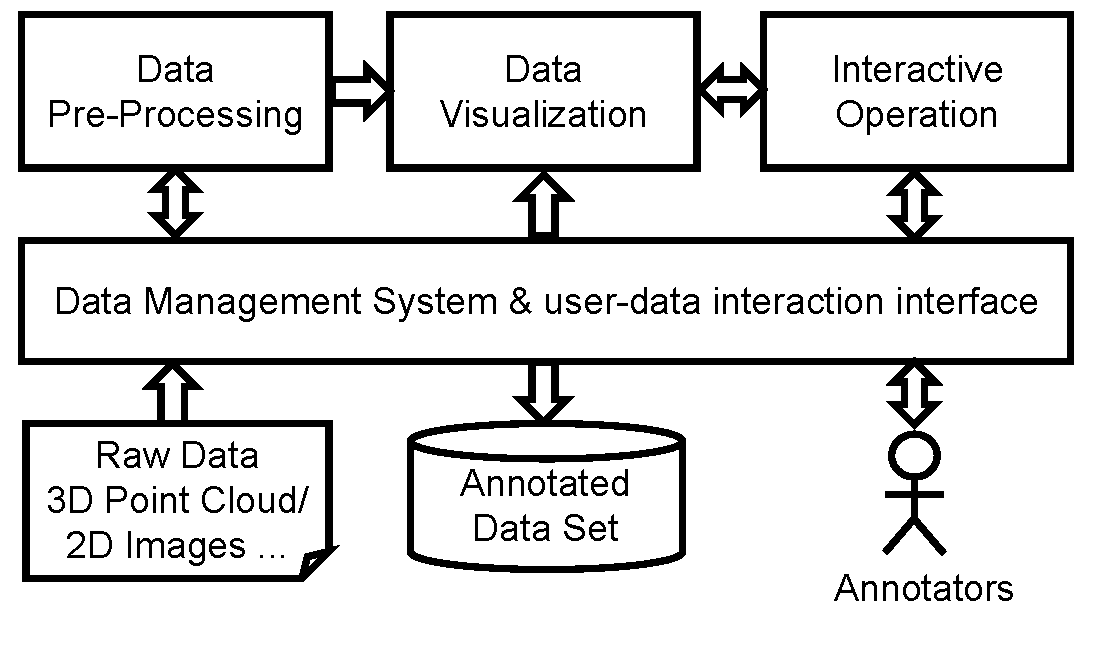
\includegraphics[width=0.45\textwidth]{./platform-simple2}\\ %\vspace{-0.3cm}
	\caption{An illustration of intelligent annotation systems for autonomous driving datasets.}
	\label{fig:main-arch}
	\vspace{-0.3cm}
\end{figure}




\begin{table*}[h]
	\caption{A comparison of 3D point cloud annotation systems in terms of visualization modules and interactive operations}
	\label{tab:comparison}
	\resizebox{1.0\textwidth}{!}{
		\begin{tabular}{c||p{1.1cm}<{\centering}|p{0.7cm}<{\centering}|p{1cm}<{\centering}|p{1cm}<{\centering}|p{1cm}<{\centering}|p{0.9cm}<{\centering}|p{1cm}<{\centering}|p{0.7cm}<{\centering}|p{1cm}<{\centering}
				||p{1cm}<{\centering}|p{1cm}<{\centering}|p{0.8cm}<{\centering}|p{1cm}<{\centering}|p{1cm}<{\centering}}
			\hline \hline
			\multirow{2}{*}{} & \multicolumn{9}{c||}{Visualization}                         & \multicolumn{5}{c}{Operation}                 \\
			\cline{2-15}                       &3D Spatial/ Temporal Navigation & Main View Focus Mode   & Box \& Object Coloring & Top/Side/ Front Views  &Photo Context with 3D-2D Fusion  &Focused Context & Mult-Camera Switching & Stream Play & Object Locking    & Box Degrees of Freedom & Auto Box Initialization& Sub-View editing &Interactive Box Fitting  & Annotation Transfer \\  \hline
			PointAtMe~\cite{pointatme}         &                 $\surd$  & $\times$               &  $\times$              &  -                     & $\surd$*                        &  $\times$      &  $\times$                       &  $\times$    &  $\times$                       & 9                      &     -                    &   n/a            &   -                 &   -            \\ \hline
			3D BAT~\cite{Zimmer20193DBA}       &                 $\surd$  & $\times$               &  $\surd *$             &  $\surd$*              & $\surd$                         &  $\times$      &  $\surd$*                       &  $\times$    &  $\times$                       & 9                      &     -                    &   -              &   -                 &   ++            \\ \hline
			LATTE~\cite{Wang2019LATTEAL}       &                 $\surd$  & $\times$               &  $\times$              &  $\times$              & $\surd$*                        &  $\times$      &  $\times$                       &  $\times$    &  $\times$                       & 5                      &     ++                   &   -              &   -                 &   ++            \\ \hline
			Supervise.ly~\cite{SUPERVISELY}    &                 $\surd$  & $\times$               &  $\surd *$             &  $\surd$               & $\surd$                         &  $\times$      &  $\times$*                      &  $\times$    &  $\times$                       & 9                      &     -                    &   ++             &   -                 &   unknwon       \\ \hline
			scale.ai~\cite{scale}              &                 $\surd$  & $\times$               &  $\surd *$             &  $\surd$               & $\surd$                         &  $\times$      &  $\surd$*                       &  $\times$    &  $\times$                       & 7                      &     unknown              &   unknown        &   -                 &   unknown       \\ \hline
			Playment.io~\cite{Playment}        &                 $\surd$  & $\times$               &  $\surd *$             &  $\surd$               & $\surd$                         &  $\times$      &  -                              &  $\times$    &  $\surd$                        & -                      &     -                    &   ++             &   -                 &   ++            \\ \hline
			\textbf{Ours}            &                 $\surd$  & $\surd$                &  $\surd$               &  $\surd$               & $\surd$                         &  $\surd$       &  $\surd$                        &  $\times$    &  $\surd$                        & 9                      &     +++                  &  +++             &  +++                &  +++            \\ \hline \hline
		\end{tabular}
	}
	\begin{tabular}{p{17.5cm}}
		
		
		The symbol ``$\surd$'' means that the system supports the functionality, ``$\times$'' means does not support,  and ``$\surd$*'' means partially supports. 
		The number of ``$\textbf{+}$''s represents the performance of a specific funcationality, more ``$\textbf{+}$''s means better performance, and ``-'' means a lack of that functionality. Some functionalities are explained as below:

		\begin{enumerate}
			\item ``Main View Focus Mode'': to zoom in and center a selected object in the main view with one click.
			
			\item ``Stream Play'': to play the sequential 3D data as a video stream
			
			\item ``Object Locking'': to automatically select the same object in all frames when the stream is playing.
			
			\item ``Focused Context'': to display the 2D image of the current object as a photo context in a single sub-view
			
			\item ``Camera Auto-Switching'': to automatically switch the photo context among multiple cameras when navigating objects.
			
			\item ``Auto Box Initialization'': to automatically fit the 3D annotation box to the whole 3D object data with one click on one point of the object data.
			
			\item ``Sub-View Editing'': to edit the 3D annotation box in one of the projective sub-views.
			
			\item ``Interactive Box Fitting'': to automatically fit the 3D annotation box to the 3D object data when editing (e.g. rotating, translating, and resizing).
			
			\item ``Annotation Transfer'': to transfer annotations across frames by an automatic or semi-automatic way.
			
		\end{enumerate}
		The meaning of other functionalities could be understood by their own names.
		
		
		
		% after \\: \hline or \cline{col1-col2} \cline{col3-col4} ...
	\end{tabular}
	\label{tab:annotationMethods}
	\vspace{-0.5cm}
\end{table*}




Current AD dataset annonation systems have developed temporal and spatial navigation tools to help quickly review annotation results \cite{Playment,SUPERVISELY,Wang2019LATTEAL,Zimmer20193DBA}, 
assigning different colors to annotation boxes to distinguish objects \cite{SUPERVISELY,Zimmer20193DBA,Playment,scale}, 
providing various perspective/projective views and multi-camera photo contexts of 3D data to help localize annotation errors \cite{SUPERVISELY,Playment,Zimmer20193DBA}, 
and supporting data stream playing and object locking in data streams to help check out the temporal consistency ammong annotation results \cite{Playment}.
However, more visualization modules such as background removal, object based coloring, and modality/spatial/temporal consistency checking should be further developed to improve the error checking efficiency.
On the other hand, interactive operations such as high degrees-of-freedom (DOFs) and multi-view editing, box initalization (one-click annotation)
and automatic fitting have also been developed \cite{pointatme,Zimmer20193DBA,Wang2019LATTEAL,SUPERVISELY,Playment}; but all need further refinement to increase annotation efficiency. 
Besides, several annotation transfer methods have been developed to achieve annotation extensions to multiple frames \cite{Playment,Wang2019LATTEAL,Zimmer20193DBA}, 
but no registration-based method has been proposed yet, which can provide more accuracy and higher speeds for annotations.


In this paper, we present a comprehensive web-based AD dataset annotation platform systems, which provide more advanced functionalities in visualization modules, interactive tools, and annotation trasnfer. The contributions of this work include
\begin{enumerate}
	\item developing an open-source portable 3D point cloud annotation platform with well-designed visualization modules and high-efficiency interactive tools, whose source codes are available for public access on Github (\url{https://github.com/naurril/SUSTechPOINTS}).
	\item developing a series of enhanced data visulization modules such as stream playing, object locking, background removal, object based coloring, multi-camera
swiching, and photo context adjusting to enable fast error checking.
	\item developing a series of new interactive tools such as smart box initialization and interactive box fitting to enable fast and accurate 3D data annotating.
	\item developing a novel registration-based inter-frame annotation transfer method, which can extend annotation results from one frame to the whole data stream with high accuracy and speeds.

\end{enumerate}


%%The platform is available for public access on github\footnote{ https://github.com/naurril/SUSTechPOINTS}.

The rest of this paper is organized as follows. 
Section~\ref{sec:realtedwork}  reviews the state-of-the-art AD dataset annotation systems and highlights the novelty of our system. 
Section~\ref{sec:systemarch} describes the system architecture and major functionalities of the proposed POINTS system. 
Section~\ref{sec:results} provides the experiment results and related discussions. 
Section~\ref{sec:conclusions} concludes the paper and outlines future work.





\begin{figure*}[t]
	
	\centering
	\vspace{-0.1cm}
	% Requires \usepackage{graphicx}
	%\resizebox{\linewidth}{!}{
	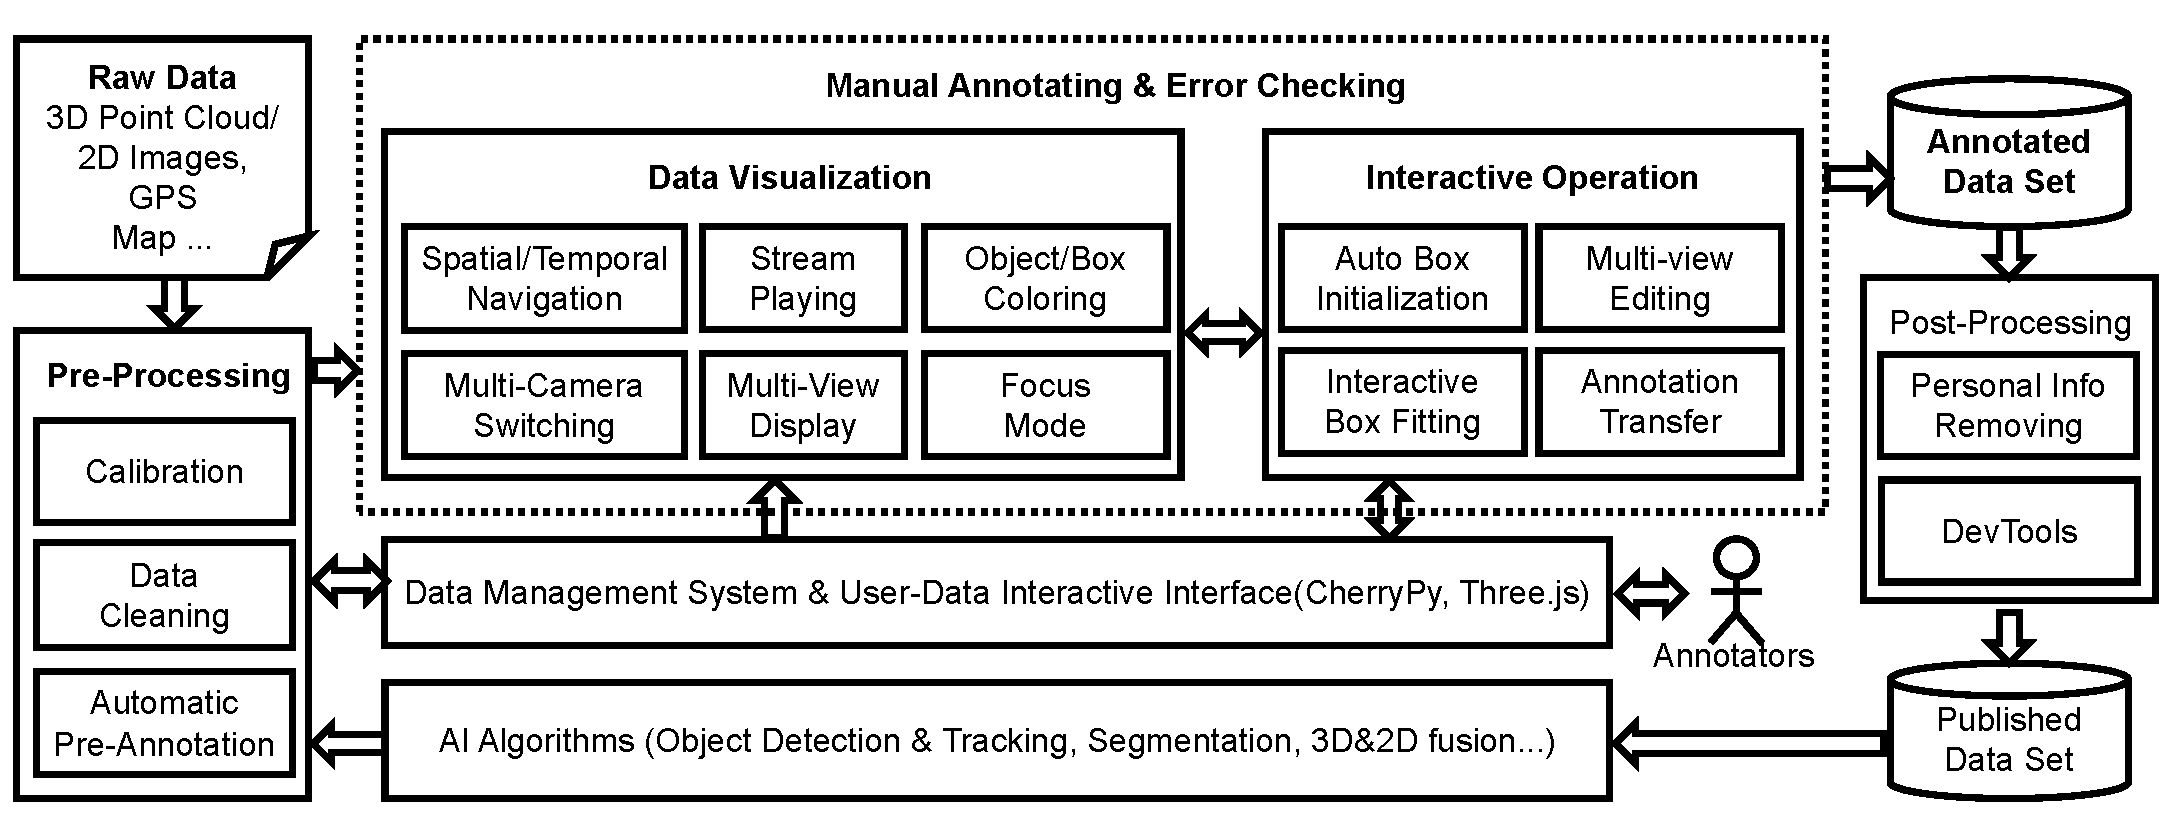
\includegraphics[width=1.0\linewidth]{./arch-big}\\ %\vspace{-0.3cm}
	\caption{The system architecture of the proposed portable point cloud interactive annotation platform system (POINTS)}
	\label{fig:arch_layer}
\end{figure*}


\section{Related work}
\label{sec:realtedwork}



Table~\ref{tab:comparison} summarizes a detailed comparison of the most popular 3D point clouds annotation systems in terms of visualization modules and interactive operations, where the first 3 systems (PointAtMe\cite{pointatme}, 3D BAT\cite{Zimmer20193DBA}, LATTE\cite{Wang2019LATTEAL}) and ours (POINTS) are open-source software, 
and the remainning 3 systems (Supervise.ly\cite{SUPERVISELY}, scale.ai\cite{scale}, Playment.io\cite{Playment}) are commercial platforms. 
It can be seen that in general the commercial platforms can provide advanced functionalities of data visualizations and interative operations, 
but their technological details are undisclosed. 
By comparison, our open-source annotation platform (POINTS) can provide unique functionalies of main view focus mode, focused context and semi
auto fitting, plus more advanced functionalities of stream playing, object locking, sub-view editing, auto box initialization and annotation transfer.

3D point cloud annotation systems can be classified as screen based and virtual-reality (VR) based. 
In the screen based systems, point clouds are visualized on 2D computer screens; users annotate objects by drawing 3D boxes with
keyboads, mouse devices and/or gestures (if touch screens are available)\cite{LabelMe3D}; camera images are displayed to help identify objects; various algorithms are developed to assist iteractive operations \cite{Wang2019LATTEAL}. 
VR based systems can provide better immersive experiences for users\cite{pointatme, gothentag}, but suffer from limits such as inaccurate operations and motion sickness. 
Therefore, in this work we choose a screen based interface to develop our annotation system.

Annotation systems can also be classified as web-based and PC-based. 
The web-based systems, such as 3D-BAT\cite{Zimmer20193DBA} and supervise.ly \cite{SUPERVISELY}, are portable for users to perform 3D object annotations only using web browsers. 
The PC-based systems, such as AppoloSuite \cite{wang2019apolloscape}, need software installed to perform annotations. 
As a result, these systems need to be updated from time to time and annotation datasets need to be downloaded from servers. 
Our proposed POINTS system is web-based, enabled by the CherryPy \cite{cherrypy} web application development framework. 
We believe that web-based systems are more portable and scalable for massive data annotating when many annotators are involved.

There are no standard benchmark metrics for annotation system evaluation yet, to the best of our knowledge.
Annotation efficiency can be measured by the annotation time used by annotators \cite{monica2017multi,pointatme,Zimmer20193DBA}. 
PointAtMe evaluates the annotation accuracy by using labor-intensive annotation results as the ground truth \cite{pointatme}. 
In this work, we choose the metrics used by PointAtMe \cite{pointatme} to evalute the efficiency and accuracy of our developed tools, 
and use its experiment results as the baseline to compare with.



III System Architecture and Module Functionalities

A. System Architecture



\section{System Architecture and Module Functionalities}
\label{sec:systemarch}

\subsection{System Architecture}

The web-based POINTS focuses on developing visualization modules and interative tools for 3D bounding box and tracking ID annotation.
The platform web server manages all the data, programmed with the CherryPy \cite{cherrypy} web application development framework.
The platform fronend provides almost all the module functionalities, programmed with the \texttt{WebGL} library, Three.js \cite{threejs}.
Fig.~\ref{fig:arch_layer} shows the system architecture of POINTS.
In the data pre-processing stage, intrinsic/extrinsic sensor parameters are estimated first; only those data frames consistent to calibration parameters, useful for algorithms training and verification are selected; then a set of AI algorithms including detection, segmentation, and 2D\&3D fusion are used to annotate the dataset initially. The data visualization modules provide helpful temporal/spatial navigation tools for users, distinguish data of different objects, and show multiple views of each object from different perspectives. The interactive data operations include editing labels in multiple views, automatically adjusting the size of 2D/3D boxes to fit the data of each object, and automatically extending (transferring) annotations of the same objects from one frame (modality) to different frames (modalities).




\subsection{Visualization}

Visualization is important for both 3D box editing and reviewing. Fig.~\ref{fig:main-ui} shows the main user interface of our platform. We describe details of visualization features in this section.

\begin{figure}[!t]
	\centering	
	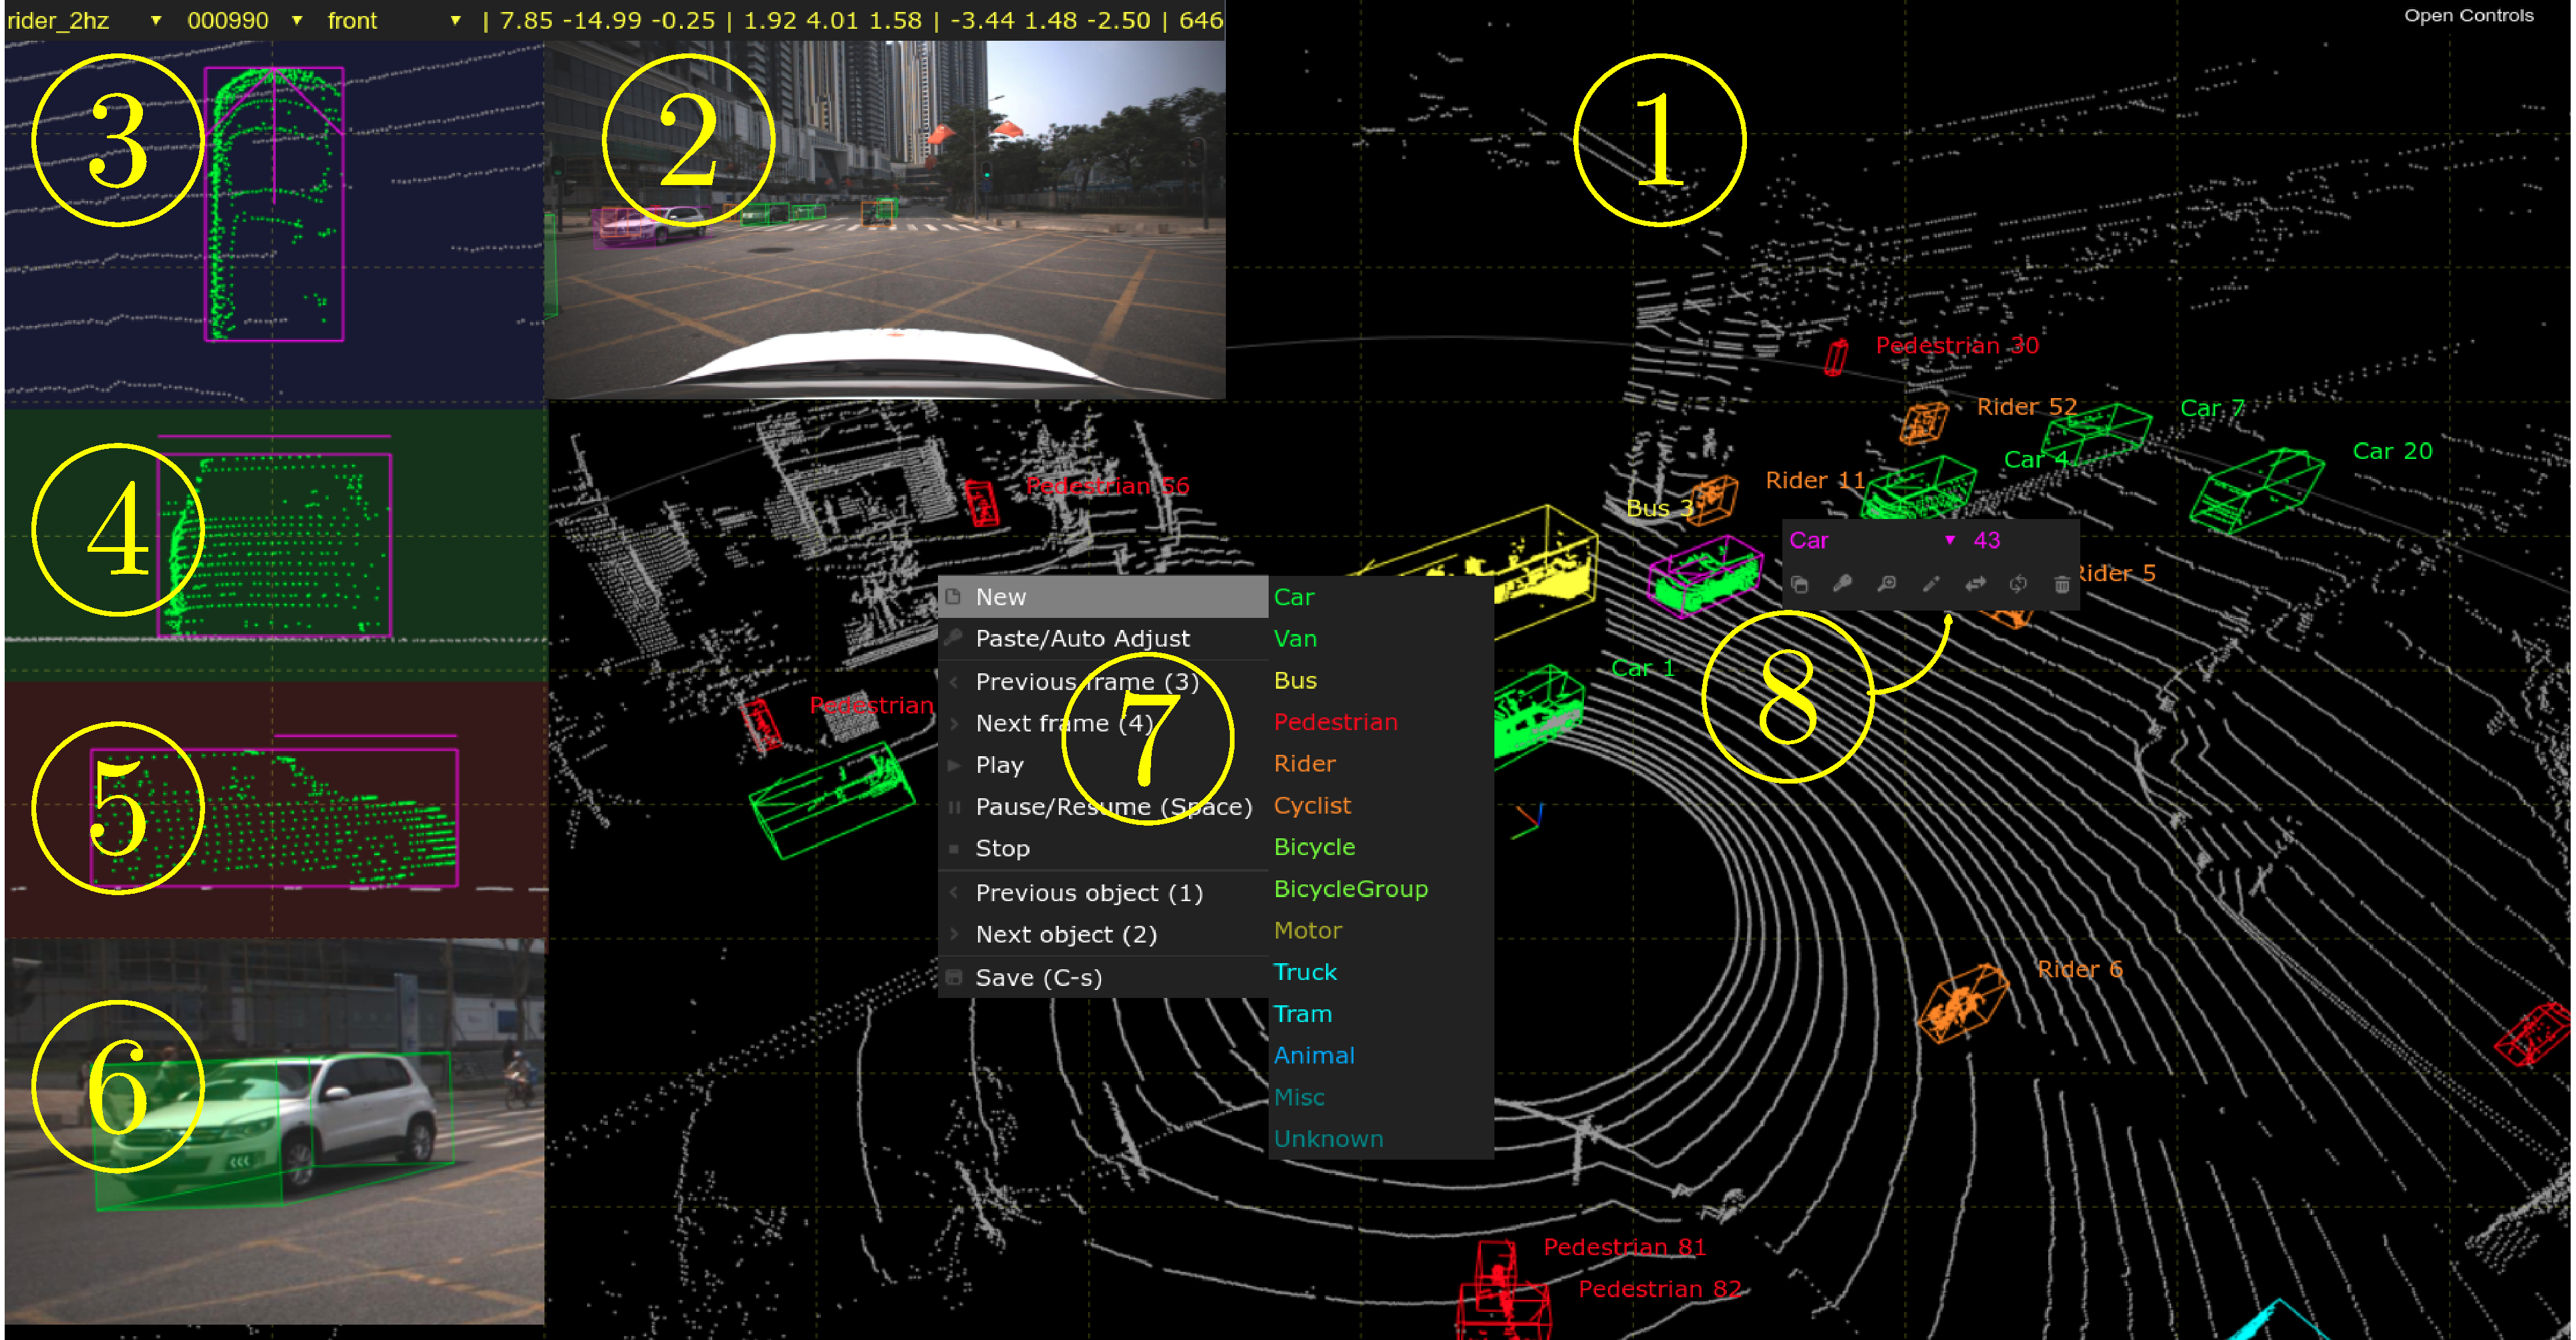
\includegraphics[width=\linewidth]{./figures/main-ui}\\
	\caption{Fig. 3: The main UI of POINTS. 
		1) the perspective view of the 3D point cloud; 
		2) the photo context, which is resizable and can be automatically switched among multiple camera images; 
		3) the top view of the selected object;
		4) the front view of the selected object; 
		5) the side view of the selected object; 
		6) the focused photo context, which can be automatically chosen for the selected object ;
		7) the context menu, which provides tools of context operations; 
		8) the floating fast toolbox, which provides most used tools.}
	\label{fig:main-ui}
\end{figure}

\subsubsection{Sub-views}
\label{section:sub-views}
We split the main window into 1 main view and 5 sub-views, as shown in Fig.~\ref{fig:main-ui}. The top,front and side projective views are displayed on left side with background hidden. Beside context photo view on the top, an extra focused context sub-view is also provided(bottom left sub-view). Annotated 3D boxes are projected to these 2 photo context sub-views.

\subsubsection{Focus-mode}
We provide a focus mode to help check object details. When activated through fast toolbox(\textcircled{8} in Fig.~\ref{fig:main-ui}),the target object is automatically centered and zoomed in, most background hidden, while all editing features still applicable. Without this feature a user has to pan,  zoom and rotate the main view often, which we think is laborious.

\subsubsection{Multi-Camera Switching}
It's common to have multiple cameras in nowadays autonomous driving car setup, \cite{Zimmer20193DBA} displays all camera images on top of the main view, some displays only one \cite{scale}. we choose the latter way but with an automatic camera switching feature. Specifically when an object is selected in point cloud, the most relevant camera image is displayed. Manual camera selection is also possible. Note that this feature needs the calibration data to be available.

\subsubsection{Object Coloring}
All boxes and object points can be colored by categories. Selected object (object under editing) are highlighted with a different color.

\subsubsection{Navigation}
\label{section:navigation}
A user can navigate in 3D space, or in time  by navigating previous or next frame. 

\subsubsection{Stream Play}
\label{section:streamplay}
A user can play the data (by scenes) like a video.

\subsubsection{Object locking}
\label{section:object-locking}
When playing, selected object are locked (\textit{i}.\textit{e}. selected in all frames).

\subsubsection{Box information}
Box details (scene, frame, object category, coordinates, dimension, direction and points number) are shown on top of the main window.
 
\subsection{Basic 3D Box Editing}

\subsubsection{Creating a box}
\label{section:create-box}
A user can create a new box by right clicking on the object  and then select object type on popup context menu. Our platform provide the following features to help create box easily:

\begin{enumerate}
	\item The initial box direction (yaw) is upright along the main view. It's common that a group of vehicles have similar or reverse directions in one scene, so adjust the view angle of the main view properly can save a lot time.
	\item A box prototype (in accordance with the object type) is placed on mouse position.
	\item A Euclidean distance based growing algorithm is invoked to include all points of the object.
	\item An auto-fitting algorithm (\ref{section:auto-fitting}) is used to shrink the box in case there is margin between the box and the object.
\end{enumerate}

Note that \emph{for most cases, the annotation is almost done with this single operation}.

Different from "one-click-annotation" of LATTE~\cite{pointatme}, which uses clustering algorithm to find points of the object under clicking, our method uses prototype to overcome difficulties when the points is too sparse for a clustering algorithm to work.

A user can also create a new box by drawing a rectangle on main view,  enclosing relevant points. The box is created by setting direction  as described above and fitted to enclosed points. The object type is automatically set by simply matching the object dimension to prototypes.


\subsubsection{Editing in perspective sub-view}

When an object is selected, a floating \emph{fast toolbox} shows next to it, as shown in Fig.~\ref{fig:main-ui}. A user can change object type, tracking id, activate focus mode, among others.

For tracking ID, A user  can input or select existing value in fast toolbox, or select 'auto' option  letting the platform to generate a new ID unique in the scene.


A user can click a selected object or the button on fast toolbox to enable box editing, drag the handlers as show in Fig.~\ref{fig:box-mouse-edit} to resize,rotate or move the box. Corresponding keyboard shortcuts are also provided.
 

\begin{figure}[t]
	\centering
 \resizebox{\linewidth}{!}{
	\begin{subfigure}{0.3\linewidth}
		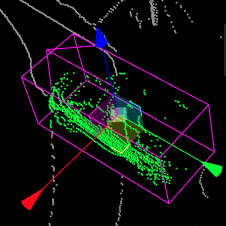
\includegraphics[height=2.5cm]{./figures/box-move}\\
		\caption{move}
	\end{subfigure}
	\begin{subfigure}{0.3\linewidth}
		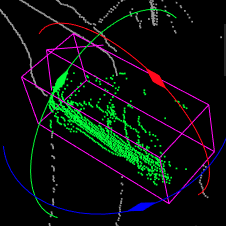
\includegraphics[height=2.5cm]{./figures/box-rotate}\\
		\caption{rotate}
	\end{subfigure}	
	\begin{subfigure}{0.3\linewidth}
		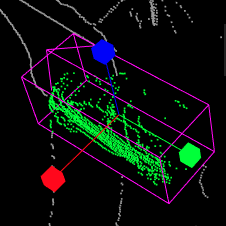
\includegraphics[height=2.5cm]{./figures/box-resize}\\
		\caption{resize}
	\end{subfigure}
}
	\caption{Box editing in perspective view}
	\label{fig:box-mouse-edit}
\end{figure}


\begin{figure}[t]
	\centering
	\resizebox{\linewidth}{!}{
		\begin{subfigure}{0.3\linewidth}
			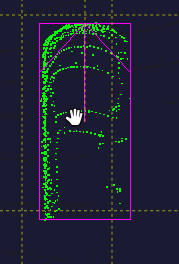
\includegraphics[height=4.cm]{./figures/subview-move-xy}\\
			\caption{move}
		\end{subfigure}
		~
		\begin{subfigure}{0.3\linewidth}
			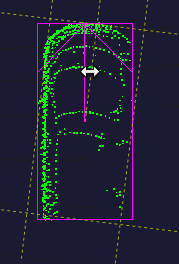
\includegraphics[height=4.cm]{./figures/subview-rotate-xy}\\
			\caption{rotate}
		\end{subfigure}
	    ~
	    \begin{subfigure}{0.3\linewidth}
	    	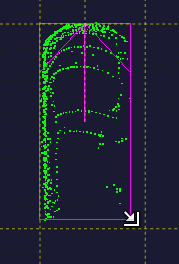
\includegraphics[height=4.cm]{./figures/subview-resize-xy}\\
	    	\caption{resize}
	    \end{subfigure}	
	}
	\caption{Box editing in projective sub-view. The dotted line shows what the box would be after the operation.}
	\label{fig:box-mouse-edit-subview}
\end{figure}

\subsubsection{Editing in projective sub-views}
Editing in perspective view is inconvenient,  a user has to change viewpoint often for better operation. As shown in Fig.~\ref{fig:main-ui} the annotation is clearly shown in the sub-views, thus we enable editing directly on these sub-views to make a better editing experience. A user can rotate, resize or move the box by mouse operation, as shown in Fig.~\ref{fig:box-mouse-edit-subview}.
All operations can also be done with keyboard shortcuts.



\subsection{Assistant algorithms}


\subsubsection{Interactive box fitting}
\label{section:auto-fitting}
When a box is being resized or rotated, our platform can fit the box to the object automatically. This is done by finding the minimal box enclosing all points. Fig.~\ref{fig:boundary-aware-rotation} shows box fitting at rotating, note all points of the object are kept inside after rotated. With this feature, \emph{to annotate a new object is as easy as to enclose all pionts first and rotate once (\ref{section:create-box})} in most cases.

Note that a direct manner to find the minimal box may fail when ground plane is present. As an example, in Fig.~\ref{fig:box-before-rotate}, if the ground plane is counted in, a new fitted box after rotation will be too large. One solution is to remove ground plane with algorithms, but it's not reliable when the ground is not smooth (as can be seen often in KITTI data set\cite{Geiger2012CVPR} where many cars parked on roadside).

We use a simple yet effective method to solve this problem. Specifically, we  ignore the most bottom part (0.2m by default) of the object when calculating the $xy$ plane dimension (width and length). Since a user is annotating the object, the pose  must be already roughly correct, so the  ground points can be removed effectively with this method. In traffic scenarios almost all objects are much higher than 0.2m, so the estimation of dimension is  seldom affected. For $z$ axis dimension (object height) we compensate the 0.2m part after the calculation. 


\begin{figure}[t]
	\centering
	
	\begin{subfigure}[t]{0.2\linewidth}
		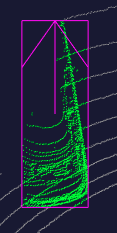
\includegraphics[height=4cm]{./figures/points-enclosed}
		\caption{}
		\label{fig:box-before-rotate}
	\end{subfigure}\hfill
	\begin{subfigure}[t]{0.2\linewidth}
		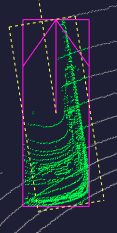
\includegraphics[height=4cm]{./figures/adjust-naively}
		\caption{}
		\label{fig:box-rotate-in-subview}
	\end{subfigure}\hfill
	\begin{subfigure}[t]{0.2\linewidth}
		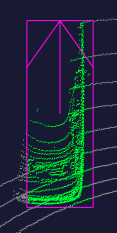
\includegraphics[height=4cm]{./figures/rotate-fail}
		\caption{}
		\label{fig:box-rotate-naively}
	\end{subfigure}\hfill
	\begin{subfigure}[t]{0.2\linewidth}
		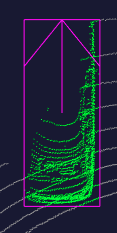
\includegraphics[height=4cm]{./figures/rotate-success}
		\caption{}
		\label{fig:box-rotate-correctly}
	\end{subfigure}\hfill
	\caption{Box auto-fitting on rotation. For box in \ref{fig:box-before-rotate}, which encloses all points of a car, if it's rotated counter-clockwise naively(\ref{fig:box-rotate-in-subview}), part of the object will go outside(left lower part of \ref{fig:box-rotate-naively}), our platform can automatically fit the box as shown in (\ref{fig:box-rotate-correctly})}
	\label{fig:boundary-aware-rotation}
	\vspace{-0.3cm}
\end{figure}


\subsubsection{Annotation transfer among related frames}
\label{semi-auto-anno}
In autonomous driving scenario, data sets are often organized by scenes\cite{Caesar2019nuScenesAM,Patil2019TheHD,lyft2019}. A scene is a sequence of frames shot at one continuous period of time. There are much similarities between neighboring frames, which makes it possible to transfer annotations among them. \cite{Zimmer20193DBA} copies annotations to next frame directly and let user do the adjustment.\cite{Wang2019LATTEAL} uses box estimation algorithm to automatically adjust the box, reusing previous annotated object size if appropriate. Our platform takes this way further by invoking registration algorithm \cite{Yang2016GoICPAG} to automatically adjust the position and rotation, reusing both the size and rotation previously annotated. In most cases our method produces  accurate enough annotation result.

A user needs to first select (copy) a reference box, then paste it at appropriate position in target frame. A registration algorithm is invoked to compute the relative transform relation between the reference and target object, then the box in the target frame is adjusted accordingly.

The reference and target objects are cropped out at a 1.2 scale ratio and all points are transformed to their corresponding box coordinates system before input to registration algorithm. Fig.~\ref{fig:annotation-transfer} shows an transfer example.

The performance of this function depends on the registration algorithm.  Empirically it works well when the reference object and the target object have similar view angles. Several adjustments may be requered if the initial position is deviated too much.

\begin{figure}[t]
	\centering
	\begin{subfigure}[t]{0.18\linewidth}
		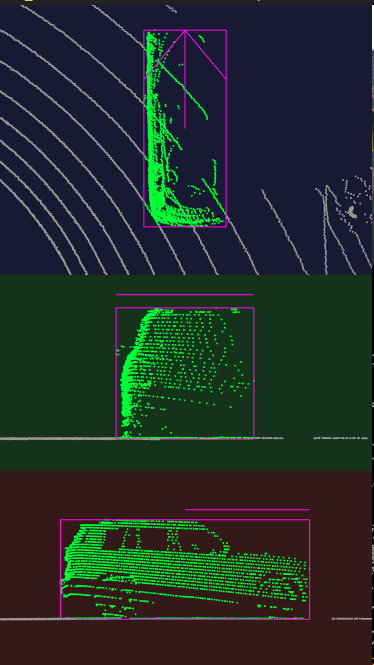
\includegraphics[height=4cm]{./figures/reg-ref-3d}\\
		\caption{}\label{fig:box-ref}
	\end{subfigure}\hfill
	~
	\begin{subfigure}[t]{0.18\linewidth}
		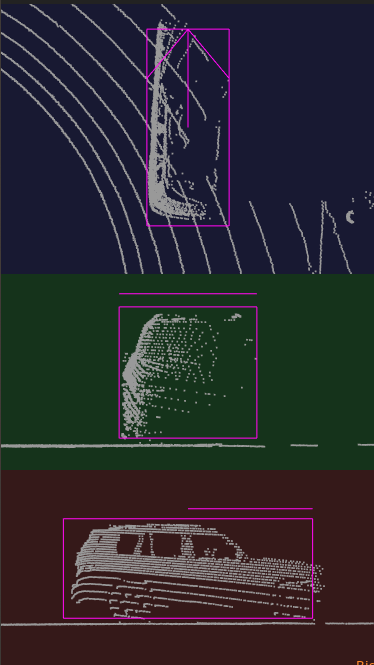
\includegraphics[height=4cm]{./figures/reg-input-3d}\\
		\caption{}\label{fig:box-source}
	\end{subfigure}\hfill
	~
	\begin{subfigure}[t]{0.18\linewidth}
		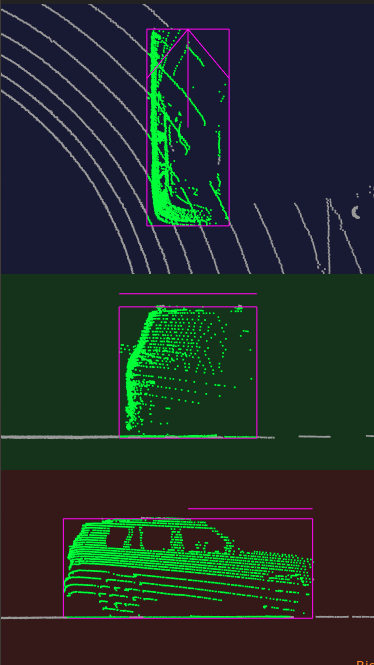
\includegraphics[height=4cm]{./figures/reg-result-3d}\\
		\caption{}\label{fig:box-output}
	\end{subfigure}\hfill
	~
	\begin{subfigure}[t]{0.18\linewidth}
		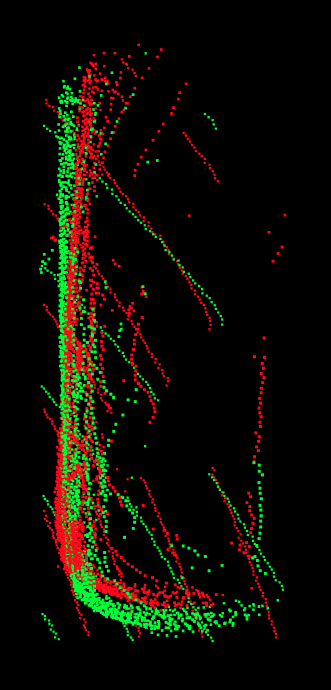
\includegraphics[height=4cm]{./figures/reg-input}\\
		\caption{}\label{fig:reg-input}
	\end{subfigure}\hfill
	\begin{comment}
	~
	\begin{subfigure}[t]{0.18\linewidth}
		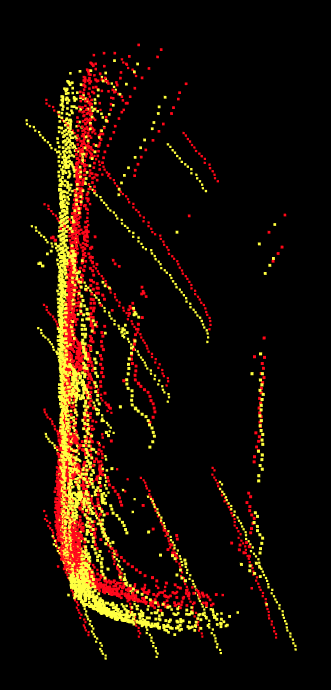
\includegraphics[height=3cm]{./figures/reg-tran}\\
		\caption{}\label{fig:reg-tran}
	\end{subfigure}\hfill
	~
	\begin{subfigure}[t]{0.18\linewidth}
		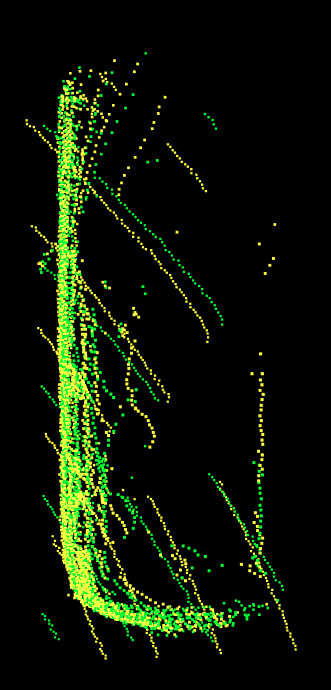
\includegraphics[height=3cm]{./figures/reg-result}\\
		\caption{}\label{fig:reg-output}
	\end{subfigure}\hfill
	\end{comment}
	
	\caption{Registration based bounding box transfer. \ref{fig:box-ref} is the reference object and its bounding box, \ref{fig:box-source} is the object in another frame with a initial  bounding box, \ref{fig:box-output} is the result of box being adjusted by annotation transfer,\ref{fig:reg-input} is the corresponding registration input after coordinates transformed.}
	\label {fig:annotation-transfer}
\end{figure}


We describe the box transformation procedure in the remaining part of this section. 
Given source and target objects (denoted by $\mathcal{S,T}$ respectively)and their bounding boxes ($b_s,b_t$), a registration algorithm finds the transform matrix $T$ to match $\mathcal{S}$ with $\mathcal{T}$ , minimizing a distance function $dist$,
$$dist(T(\mathcal{S}),\mathcal{T})$$
where we represent points of $\mathcal{S,T}$ in their corresponding bounding box coordinates $B_s$ and $B_t$, the world coordinate system is denoted as $B_w$. Note that the box itself is identical to box coordinates system (\textit{i}.\textit{e}. $b_s$ is identical to $B_s$) since we concern only the rotation (correspond to 3 axes) and position (correspond to the origin point) of the box.

Assume point $s \in \mathcal{S}$ corresponds to $t \in \mathcal{T}$ after registration, then


\begin{align}
T s^{B_s} &= t^{B_t}\\
T B_s^{-1}s^{B_w} &= t^{B_t} \label{eq:eq1}
\end{align}

where $s^{B_s}$ means s represented in $B_s$ coordinate system.

If we denote the new coordinate system of $\mathcal{S}$ as $B'_s$, then
\begin{align} 
s^{B'_s} &= t^{B_t}\\
(B'_s)^{-1}s^{B_w} &= t^{B_t} \label{eq:eq2}
\end{align}


by Eq.~\eqref{eq:eq1} and Eq.~\eqref{eq:eq2}, we have

\begin{align}
{B'_s} & = (T B_s^{-1})^{-1}\\
       & = B_s T^{-1} \label{eq:eq5}
\end{align}

If we use the reference object as target, object under annotation as source, Eq.~\eqref{eq:eq5} tells us we should apply the reverse transform of registration to the coordinates system, that is, to the box.


%\subsection{Proposed annotation procedure}

\section{Results and Evaluation}
\label {sec:results}

The evaluation consists of 3 parts:
\begin{enumerate}
	\item Evaluation of review efficiency, we show that errors or inaccuracies are easy to identify through the visualization functionalities.
	\item Evaluation of annotation efficiency, we show that annotation time and accuracy is better compared to other available tools.
	\item Evaluatoin of transfer annotation, we show that transfer annotation generate accurate enough results.
\end{enumerate}

\subsection{Review Efficiency}
We use examples from KITTI 3D Object Detection data set \cite{Geiger2012CVPR}  to demonstrate the effectiveness of checking annotation accuracy with our platform. We choose the same scene as show in  Fig. 5 of \cite{pointatme}.

Note although our platform supports all 9 degrees of freedom for 3D box, only 7 are labeled in KITTI data set, with pitch and tilt ignored, so in our evaluation we also ignore these 2 angles for fairness.

As show in Fig.~\ref{fig:annocheck}, we demonstrate that thanks to the 4 sub-views (Section~\ref{section:sub-views}) errors or inaccuracy spots are immediately and clearly identified by just navigating the objects one by one (Section~\ref{section:navigation}).

Tracking IDs can also be easily checked with the help of object locking (\ref{section:object-locking})  and stream-play(\ref{section:streamplay}) feature. For brevity we choose not to show examples here.

\begin{figure}
	\centering
	\begin{subfigure}{0.3\linewidth}
		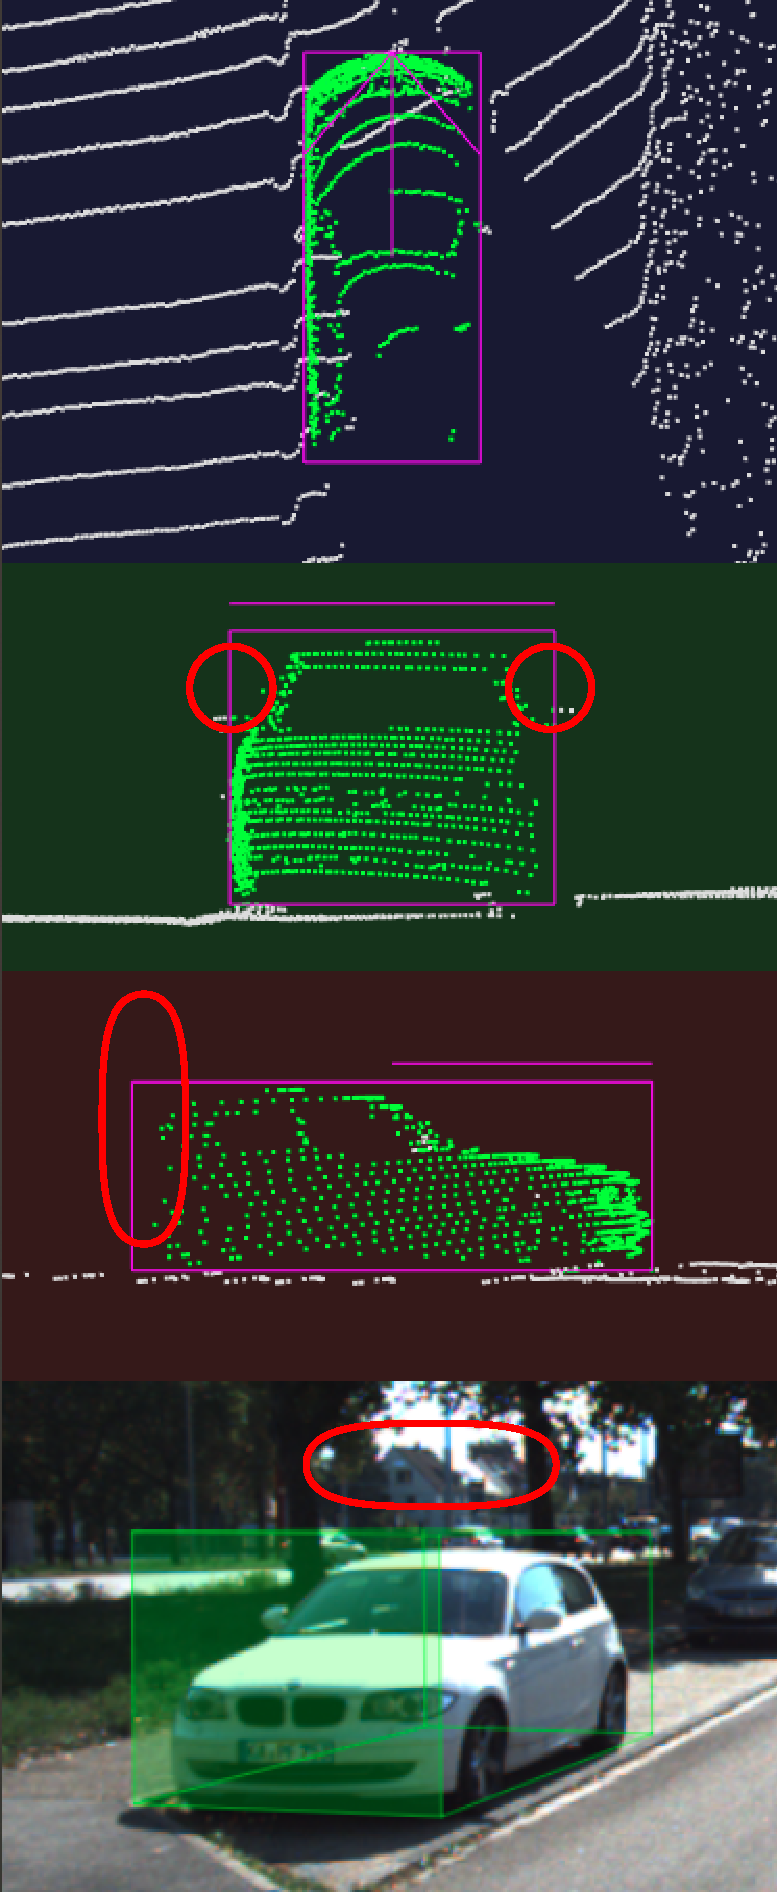
\includegraphics[scale=0.2]{./figures/annocheck-0}
	\end{subfigure}
	~
	\begin{subfigure}{0.3\linewidth}
		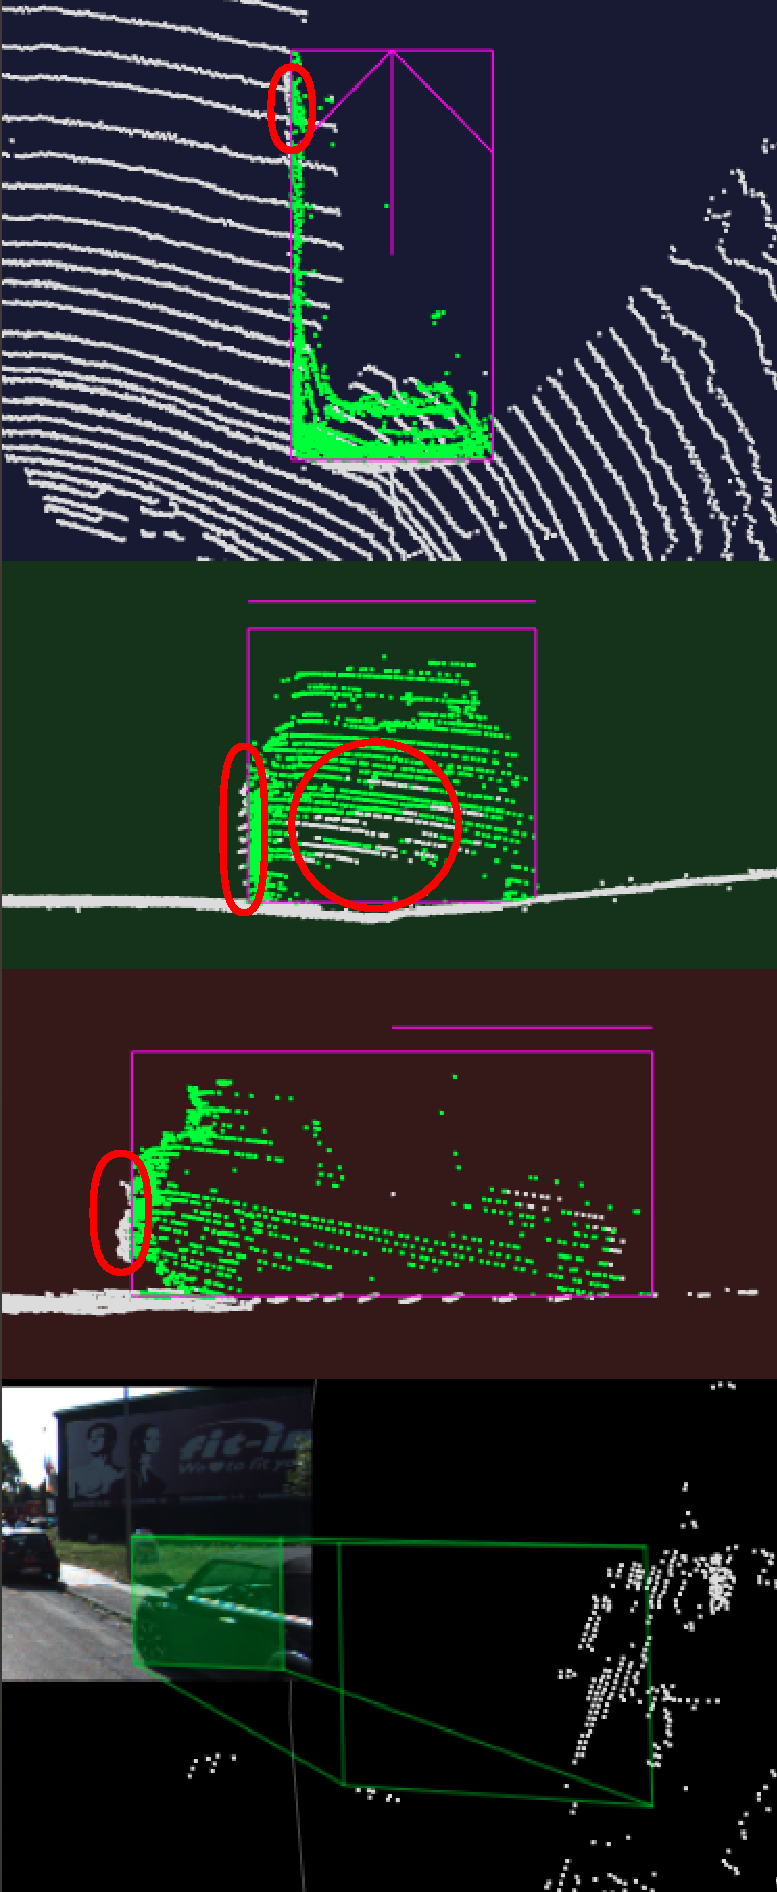
\includegraphics[scale=0.2]{./figures/annocheck-1}
	\end{subfigure}
	~
	\begin{subfigure}{0.3\linewidth}
		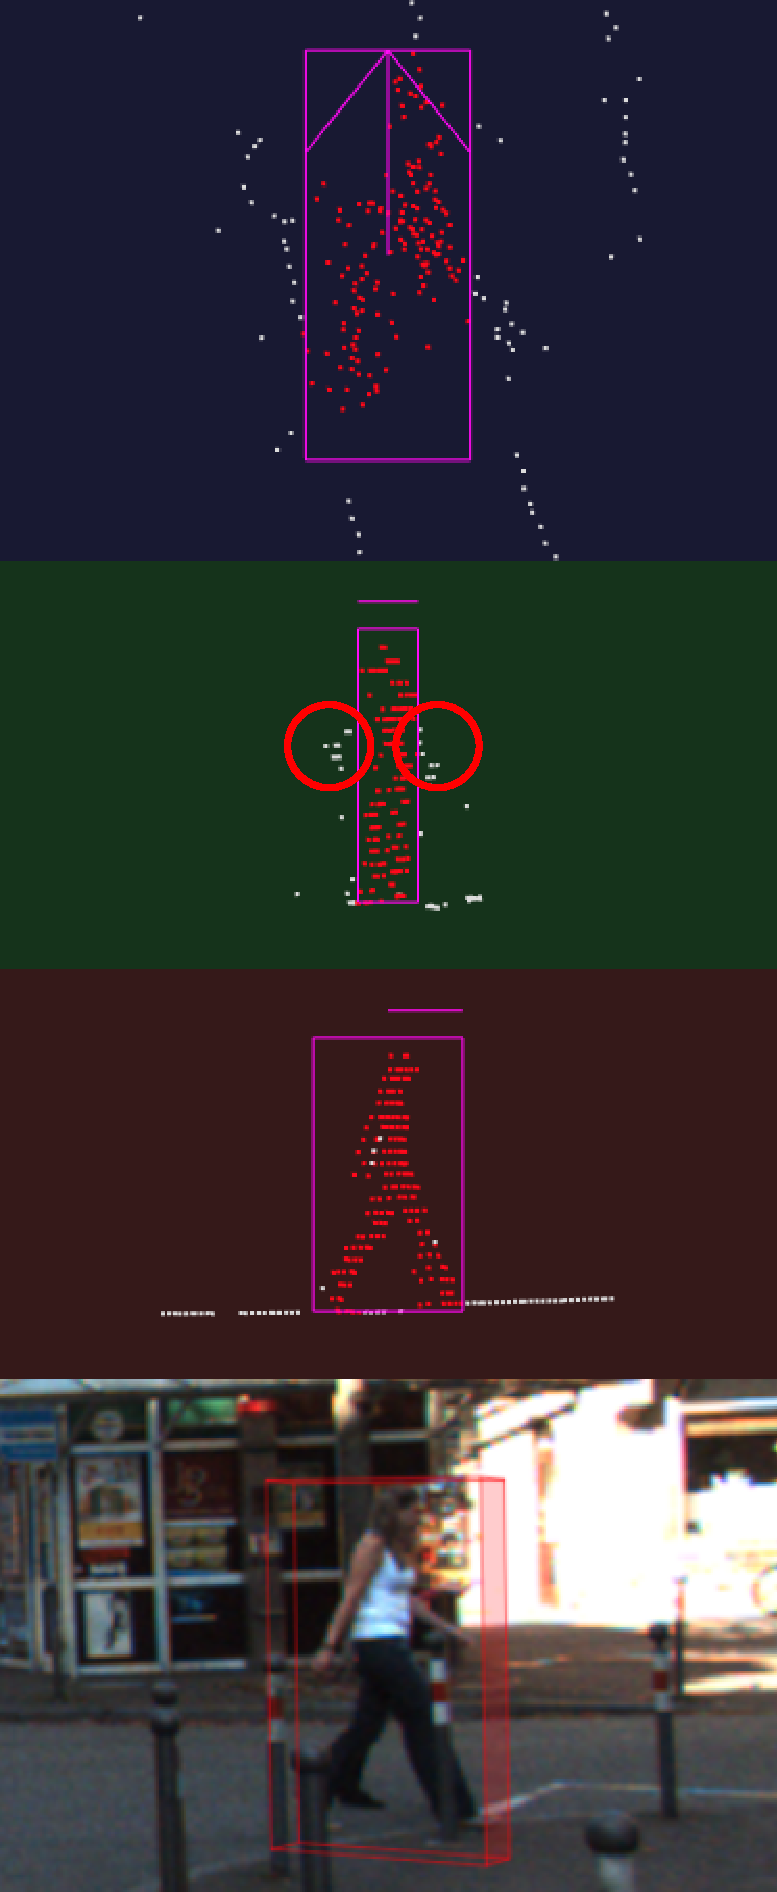
\includegraphics[scale=0.2]{./figures/annocheck-2}
	\end{subfigure}
	
	\caption{Checking inaccuracies in KITTI 3D object detection data set}
	\label{fig:annocheck}
\end{figure}


\subsection{Object Annotating}

Annotation efficiency can be measured by annotation time and accuracy\cite{pointatme} \cite{Zimmer20193DBA}. The time shall be minimized and accuracy maximized. \cite{Zimmer20193DBA} counts interpolated annotations in so the time per object is extremely small, for fairness we use \cite{pointatme} as the baseline to compare our platform with.

As described in \cite{pointatme} and also indicated in previous section, the original KITTI labels are not suited as ground truth for our benchmarks. So we carefully annotated some scenes and use the result as ground truth, 3 users are employed to annotate the same set of data, with a few hours of practicing beforehand. We choose the same scene as used in \cite{pointatme}. For ground truth annotation the average time used per object is less than 20 seconds.

For accuracy evaluation we follow the criteria  described in \cite{pointatme}, all points belonging to an object should be inside the bounding box and all points not belonging to it should be outside.
The test result is show in Table~\ref{tab:annotation-evaluation}.
\begin{table}[h]
	\centering
	\caption{Results compared with baseline}
	\label{tab:annotation-evaluation}
	\begin{tabular}{|l|c|c|c|c||c|c|c|c|}
		\hline
		\textbf{Method} & \textbf{Ours} & \textbf{PointAtME\cite{pointatme}} \\
		\hline
		\hline
		Time/Object (sec.) & 24 $\pm$ 6 & 55.2 $\pm$ 12.1\\
		\hline
		Undo/Object & - & 0.42 $\pm$ 0.43\\
		\hline
		Errors (Points/Object) & $<$1 & 28.7 $\pm$ 5.1\\
		\hline
		FP ratio / Object & - & 7.16\%\\
		\hline
		FN ratio / Object & - & 3.27\%\\
		\hline
	\end{tabular}
\end{table}


\subsection{Annotation transfer}
For annotation transfer we evaluate the accuracy. We  transfer annotations between frames that have 0.5 to 2.5 second difference in time, with our self-collected data set. The result is shown in Table~\ref{tab:transfer-evaluation}.



\begin{table}[h]
	\centering
	\caption{Accuracy of transfer annotations}
	\label{tab:transfer-evaluation}
	\begin{tabular}{|c|r|c|c|c|c|c|}
		\hline
		 & \textbf{Obj Type} & \textbf{Ref. Obj.}&\textbf{0.5s} & \textbf{1s} & \textbf{1.5s}& \textbf{2.5s} \\
		\hline
		\hline
		 1 & Car &-/1958& 15/1372 & 25/910 & 19/658 &  1/388\\
		\hline
  		 2 & Rider &-/329& 0/240 & 0/190 & 0149/658 &  0/94\\
		\hline
  		 3 & Bus &-/2327& 5/1208 & 3/656 & 1/396 &  0/244\\
\hline
	\end{tabular}

\begin{tabular}{p{\linewidth}}
	The content is Error/Total points. `Ref. Obj.` means reference object (i.e. manually annotated object)
\end{tabular}


\end{table}


\section{CONCLUSIONS}
\label{sec:conclusions}

We introduced a novel 3D object annotation platform, focusing on visualization, operations and assisting algorithms. We demonstrated with tests that our platform can improve annotation accuracy with greater efficiency compared to other tools. The future direction will be to integrate more algorithms, for example, to integrate object tracking algorithm to work with our novel annotation transfer method to make our platform more efficient.



\addtolength{\textheight}{-12cm}   % This command serves to balance the column lengths
                                  % on the last page of the document manually. It shortens
                                  % the textheight of the last page by a suitable amount.
                                  % This command does not take effect until the next page
                                  % so it should come on the page before the last. Make
                                  % sure that you do not shorten the textheight too much.

%%%%%%%%%%%%%%%%%%%%%%%%%%%%%%%%%%%%%%%%%%%%%%%%%%%%%%%%%%%%%%%%%%%%%%%%%%%%%%%%



%%%%%%%%%%%%%%%%%%%%%%%%%%%%%%%%%%%%%%%%%%%%%%%%%%%%%%%%%%%%%%%%%%%%%%%%%%%%%%%%



%%%%%%%%%%%%%%%%%%%%%%%%%%%%%%%%%%%%%%%%%%%%%%%%%%%%%%%%%%%%%%%%%%%%%%%%%%%%%%%%
\begin{comment}


\section*{APPENDIX}

\subsection{Raw data orgnization}
In server, the raw data is organized by scenes, the directory structure is as in Fig.~\ref{fig:data-dir}.

\begin{figure}

	\dirtree{%
		.1 data.
		.2 scene1.
		.3 lidar.
		.4 frame0000.pcd.
		.4 ....
		.3 image.
		.4 left-camera.
		.5 frame0000.png.
		.5 ....
		.4 front.
		.5 frame0000.png.
		.5 ....
		.4 ....
		.3 calib.
		.4 left-camera.json.
		.4 front.json.
		.4 ....
		.3 label.
		.5 frame0000.json.
		.5 ....
		.2 scene2.
		.3 ....
		.2 ....
	}
	\caption{Raw data organization. The `label` folder is used to store annotation result. the `calib` folder stores lidar-camera calibration parameters, which is optional but requrired for 3d-2d fusion features. We list 3 cameras as an example, more cameras are also supported.}
	\label{fig:data-dir}
\end{figure}


\subsection{Operation summary}
\label{app:operations}
Table~\ref{table:keyboard_mainview} shows operations applicable in main view, Table~\ref{table:keyboard_subview} show operations applicable in side sub-views.

\begin{table}[h]
	\caption{Operations on main-view}
	\label{table:keyboard_mainview}
	\begin{center}
		\begin{tabular}{|c|l|}
			\hline
			\textbf{Key} & \textbf{Function}\\
			\hline
			1 & select previous object\\
			\hline
			2 & select next object\\
			\hline
			3 & previous frame\\
			\hline
			4 & next frame\\
			\hline
			r & rotate counterclockwise(yaw)\\
			\hline
			f & rotate clockwise(yaw)\\
			\hline
			t & reset box\\
			\hline
			g & reverse direction (yaw angle)\\
			\hline
			v & switch editing mode(Fig.~\ref{fig:box-mouse-edit})\\
			\hline
			Ctrl+s & save\\
			\hline
			Ctrl+c & copy reference box (\ref{semi-auto-anno})\\
			\hline
			Ctrl+z & undo\\
			\hline
			Ctrl+y & redo\\
			\hline
			Left drag & rotate view\\
			\hline
			Right drag & pan view\\
			\hline
			Wheel up & zoom in\\
			\hline
			Wheel down & zoom out\\
			\hline
			Ctrl+Left Drag (on main view)& mark points\\
			\hline
			Ctrl+Left click (on photo context)& draw polygon\\
			\hline
		\end{tabular}
	\end{center}
\end{table}


\begin{table}[h]
	\caption{Operations on sub-views}
	\label{table:keyboard_subview}
	\begin{center}
		\begin{tabular}{|c|l|c|l|}
			\hline
			\textbf{Key} & \textbf{Function}\\			
			\hline
			a & move left\\
			\hline
			s & move down\\
			\hline
			d & move right\\
			\hline
			w & move up\\
			\hline
			q & rotate left\\
			\hline
			e & rotate right\\
			\hline
			q & rotate left\\
			\hline
			e & rotate right\\
			\hline				
			Ctrl-q & rotate left with boundary aware\\
			\hline
			Ctrl-e & rotate right with boundary aware\\
			\hline
			Drag box border/corner & resizing box\\
			\hline
			Drag direction line & rotate box\\
			\hline
			Drag box border/corner with Ctrl hold & resizing box with auto-shrink\\
			\hline
			Drag direction line with Ctrl hold& rotate box with boundary aware\\
			\hline
			Drag box center & move box\\
			\hline
			Double click box border/corner & auto-shrinking\\
			\hline
			Double click box center & auto-shrinking all borders\\
			\hline
			Double click direction line& rotate upside-down (180 degree)\\
			\hline
		\end{tabular}
	
		 {\raggedright Note that all operation effects are relative to current sub-view.\par}
		 
	\end{center}
\end{table}
\section*{ACKNOWLEDGMENT}


\end{comment}

%%%%%%%%%%%%%%%%%%%%%%%%%%%%%%%%%%%%%%%%%%%%%%%%%%%%%%%%%%%%%%%%%%%%%%%%%%%%%%%%


\bibliographystyle{IEEEtran}
\bibliography{MyReference}
\end{document}
